\documentclass[11pt,compress,t,notes=noshow, aspectratio=169, xcolor=table]{beamer}

\usepackage{../../style/lmu-lecture}
% Defines macros and environments
% This file is included in slides and exercises

% Rarely used fontstyle for R packages, used only in 
% - forests/slides-forests-benchmark.tex
% - exercises/single-exercises/methods_l_1.Rnw
% - slides/cart/attic/slides_extra_trees.Rnw
\newcommand{\pkg}[1]{{\fontseries{b}\selectfont #1}}

% Spacing helpers, used often (mostly in exercises for \dlz)
\newcommand{\lz}{\vspace{0.5cm}} % vertical space (used often in slides)
\newcommand{\dlz}{\vspace{1cm}}  % double vertical space (used often in exercises, never in slides)
\newcommand{\oneliner}[1] % Oneliner for important statements, used e.g. in iml, algods
{\begin{block}{}\begin{center}\begin{Large}#1\end{Large}\end{center}\end{block}}

% Don't know if this is used or needed, remove?
% textcolor that works in mathmode
% https://tex.stackexchange.com/a/261480
% Used e.g. in forests/slides-forests-bagging.tex
% [...] \textcolor{blue}{\tfrac{1}{M}\sum^M_{m} [...]
% \makeatletter
% \renewcommand*{\@textcolor}[3]{%
%   \protect\leavevmode
%   \begingroup
%     \color#1{#2}#3%
%   \endgroup
% }
% \makeatother


\newcommand{\gh}{\hat{g}}
\title{Interpretable Machine Learning}
% \author{LMU}
%\institute{\href{https://compstat-lmu.github.io/lecture_iml/}{compstat-lmu.github.io/lecture\_iml}}
\date{}

\begin{document}
	
	% Set style/preamble.Rnw as parent.
	
	% Load all R packages and set up knitr
	
	% This file loads R packages, configures knitr options and sets preamble.Rnw as 
	% parent file
	% IF YOU MODIFY THIS, PLZ ALSO MODIFY setup.Rmd ACCORDINGLY...
	
	% Defines macros and environments
	
	\newcommand{\titlefigure}{figure/lime5}
    \newcommand{\learninggoals}{
    	\item Learn why LIME should be used with caution
    	\item Possible pitfalls of LIME}
	
	\lecturechapter{LIME Pitfalls}
	\lecture{Interpretable Machine Learning}
	
	% Prerequisite: le-into, le-lime
	
	% ------------------------------------------------------------------------------


\begin{frame}{LIME Pitfalls}
  \begin{itemize}
  	\item %Despite being a popular interpretation method, several papers caution to be careful in LIME
  	LIME is one of the most widely used methods for local interpretability\\ 
  	$\leadsto$ But several papers highlight important (practical) limitations
  	\item Pitfalls arise at multiple levels, which will be discussed in detail:
    \begin{itemize}
  \item \textbf{Sampling} -- ignores feature dependencies, risks extrapolation
  \item \textbf{Locality definition} -- kernel width and distance metrics affect sensitivity
  \item \textbf{Local vs. global features} -- global signals may overshadow local ones
  \item \textbf{Faithfulness} -- trade-off between sparsity and local accuracy
  \item \textbf{Hiding biases} -- explanations can be manipulated to appear fair
  \item \textbf{Robustness} -- explanations vary for similar points
  \item \textbf{Superpixels (images)} -- instability due to segmentation method
\end{itemize}
  	% \begin{itemize}
  	%     \item Sampling procedure (extrapolation)
  	%     \item Definition of locality (sensitivity)
  	%     \item Scope of feature effects (local vs. global)
  	%     \item Faithfulness (trade-off with sparsity)
  	%     \item Surrogate model (hiding biases, robustness)
  	%     \item Definition of superpixels in case of image data (sensitivity)
  	% \end{itemize}
  	%\item These are discussed in more detail in the following 
  \end{itemize}
  
\end{frame}
  
\begin{frame}{Pitfall: Sampling}
	\begin{itemize}
	\itemsep1em
	  \item \textbf{Pitfall}: Common sampling strategies for $\zv \in \Zspace$ ignore feature dependencies
      % \item \textbf{Implication}:  Unlikely data points might be used to learn local explanation models
        \item \textbf{Implication:} Surrogate model may be trained on unrealistic points\\
  $\leadsto$ Undermines the fidelity and validity of the explanation
      \pause
      \item \textbf{Solution I}: Sample locally from the true data manifold $\Xspace$\\
  $\leadsto$ Challenging in high-dimensional or mixed-type data settings
      \item \textbf{Solution II}: Restrict sampling to training data near $\xv$\\
      $\leadsto$ Requires enough training data points near $\xv$
    \end{itemize}
    
\end{frame}

\begin{frame}{LIME Pitfall: Locality}

	\begin{itemize} 
     \item \textbf{Pitfall}: Difficult to define locality (= how samples are weighted locally) %\\
    % \begin{itemize}
     %    \item[$\leadsto$] 
     %$\leadsto$ Strongly affects local model, but there is no automatic procedure for choosing neighborhood
     %\end{itemize}
     \item \textbf{Implication:} Local model and explanation quality depend heavily on this weighting, but no principled way exists to choose it

     \item \textbf{Default:} Use exponential kernel as proximity measure between $\xv$ and $\zv$:\\
     	$\neigh(\zv) = exp(-d(\xv, \zv)^2/\sigma^2)$ with distance measure $d$ and kernel width $\sigma$
    %  	 \begin{center}
    %  		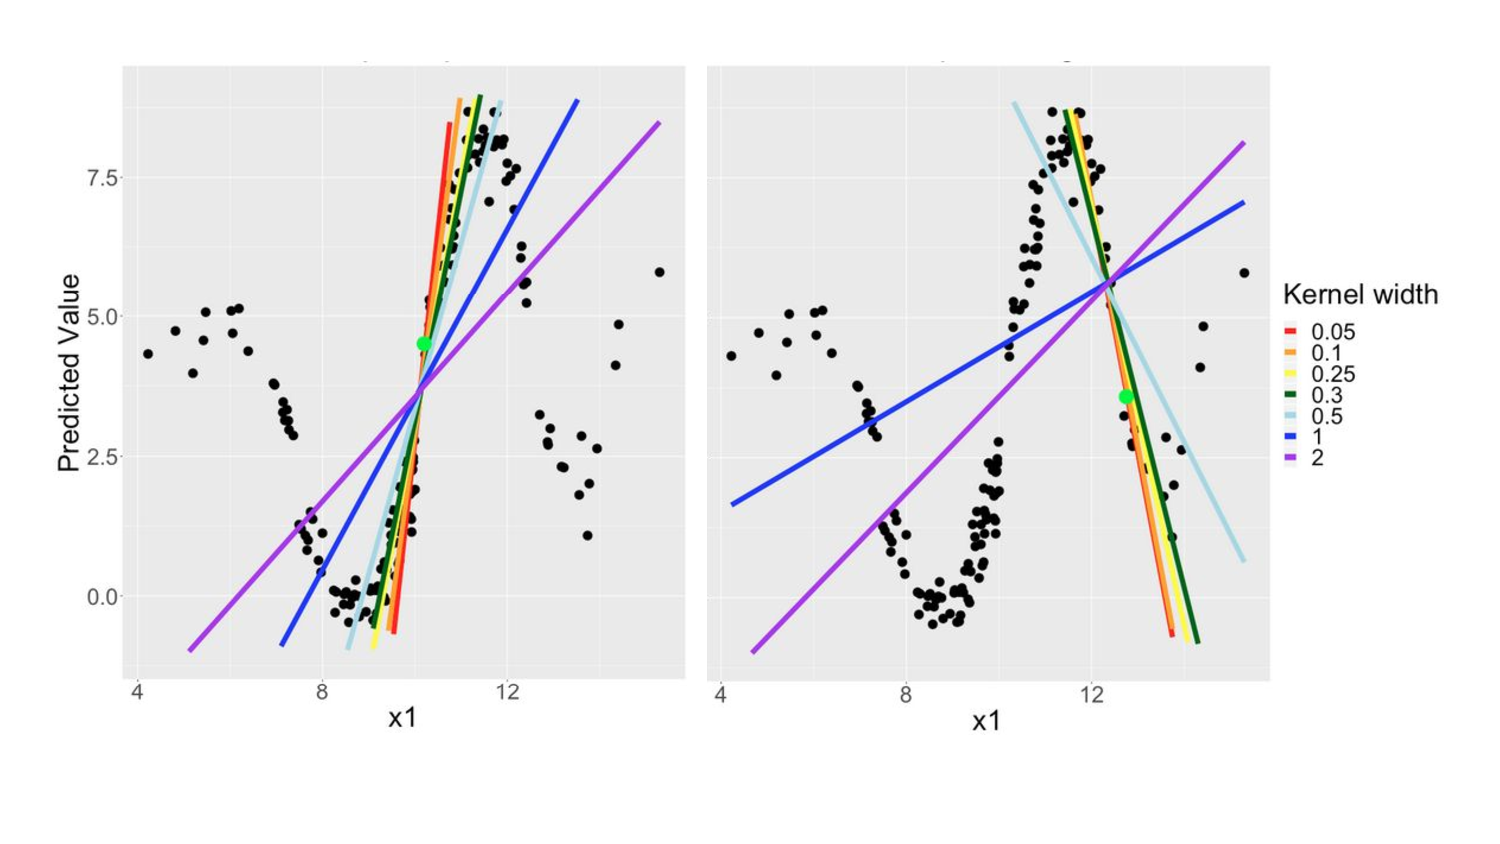
\includegraphics[width=0.6\textwidth]{figure/lime_locality}
    %  		\vspace{-0.5cm}
     		
    %  		\scriptsize{Linear surrogate models for two observations based on the same model with one target and one feature. Each line displays one linear surrogate model with different kernel width. In the right figure, larger kernel sizes are more severe.}
     		
    %  	\end{center}
     \end{itemize}
     \pause
     \textbf{Example:} For 2 obs. (green points), fit local surrogate models (lines) using only \( x_1 \)
     \begin{columns}[T, totalwidth=\textwidth]
        \begin{column}{0.72\textwidth}
        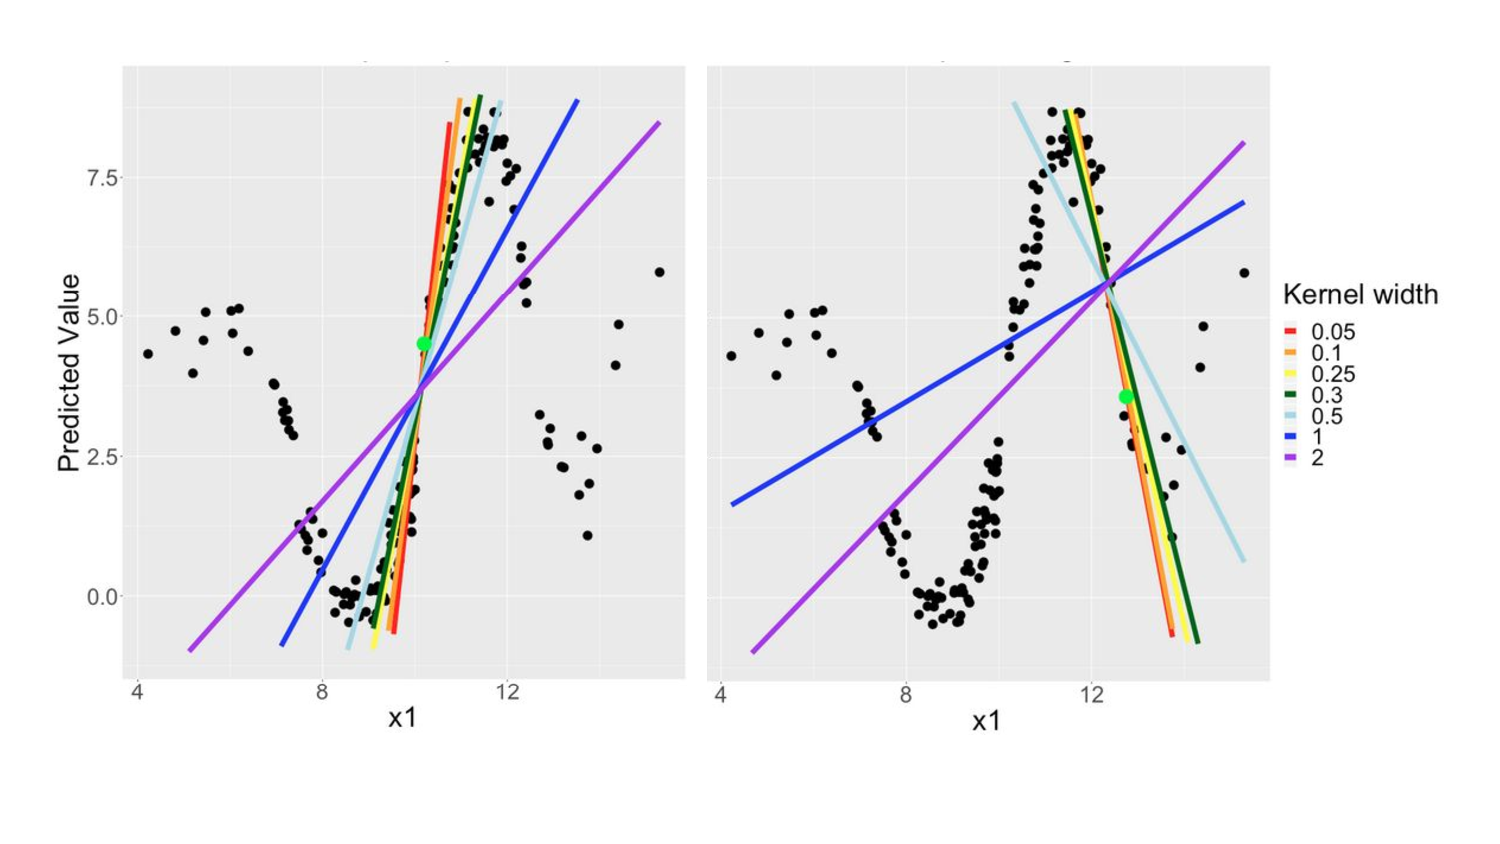
\includegraphics[width=\textwidth, trim = 25px 0px 15px 40px, clip]{figure/lime_locality}
         \end{column}
         \begin{column}{0.28\textwidth}
         % \begin{itemize}
         %     \item Surrogate models for 2 obs. (green points) for same model with one feature $x_1$
         %     \item Each line refers to a linear surrogate model with different kernel width
         %     \item Right figure: larger kernel widths influence lines more
         % \end{itemize}
         %\begin{itemize}
  %\item 
    \lz
  \textbf{Line colors:} different kernel widths used for proximity weighting\\
  \lz
  %\item 
  \textbf{Right:} larger kernel widths affect lines more
%\end{itemize}

         \end{column}
     \end{columns}
\end{frame}

\begin{frame}{LIME Pitfall: Locality \citebutton{Kopper et al. 2019}{https://slds-lmu.github.io/iml_methods_limitations/}}
%     \begin{itemize} 
%          \item \textbf{Solution I}: Kernel width strongly interacts with locality:
%          \begin{itemize}
%              \item Large kernel width leads to interaction with points further away (unwanted)
%              \item Small kernel width leads to small neighborhood\\
%              $\leadsto$ risk of few data points\\
%              $\leadsto$ potentially fitting more noise
%          \end{itemize}
%          \pause
%     	\item \textbf{Solution II}: Use Gower distance where no kernel width needs to be specified 
%     	\begin{itemize}
%     	    \item \textbf{Problem}: data points far away receive weight $ > 0$\\
%     	    $\leadsto$ resulting explanations are rather global than local surrogates   
%     	\end{itemize}
%     \end{itemize}
% \vspace{0.3cm}

\begin{itemize}
  \item \textbf{Pitfall:} Choice of kernel width (\(\sigma\)) critically influences locality
  \pause
  \item \textbf{Implication of edge cases:}
  \begin{itemize}
    \item \emph{Large} $\sigma$ $\rightarrow$ overemphasize distant points, hurting locality
    \item \emph{Small} $\sigma$ $\rightarrow$ risk of too few points, leading to unstable or noisy explanations
  \end{itemize}
  \pause
  \item  \textbf{Solution I:} Use Gower similarity directly as weights: \( \pi(\zv) = 1 - d_{\text{Gower}}(\xv, \zv) \)\\
  $\leadsto$ No kernel width required, but distant points still receive (too high) weight\\
  $\leadsto$ Explanation may reflect more global than local structure\\
  $\leadsto$ Used in practical LIME implementations \citebutton{lime package}{https://goodekat.github.io/LIME-research-journals/journals/02-understanding_lime/02-understanding_lime.html}
  \pause
  \item \textbf{Solution II:} s-LIME adaptively selects \(\sigma\) to balance fidelity and stability \citebutton{Gaudel et al. 2022}{https://arxiv.org/abs/2208.01510}
\end{itemize}
\end{frame}

\begin{frame}{Pitfall: Local vs. Global Features \citebutton{Laugel et al. 2018}{https://arxiv.org/pdf/1806.07498.pdf}}

\begin{itemize}%[<+->]
	\item<1-> \textbf{Pitfall:} Sampling from entire input space may hide influence of locally relevant features in favor of globally relevant ones, even for narrow kernels.
 \item<1-> \textbf{Feature types:}
  \begin{itemize}
    \item \emph{Global features} influence predictions broadly across whole imput space $\Xspace$
    \item \emph{Local features} affect predictions only in small subregions of $\Xspace$
  \end{itemize}
  
  \item<2-> \textbf{Implication:} LIME’s surrogate may over-weight global features, producing explanations that miss critical local signals.
	% \item<2-> \textbf{Implication}: 
	% \begin{itemize}
 %        \item \emph{Global features:} influence predictions broadly across $\Xspace$
 %    \item \emph{Local features:} affect predictions only in small subregions
	%     % \item Some features influence the \textbf{global} shape of the black-box model
	%     % \item Other \textbf{local} features impact predictions only in smaller regions of $\Xspace$ %for a small area of $\Xspace$ 
	% \end{itemize}
	\item<3-> \textbf{Example}: Decision trees
    \begin{itemize}
        \item Features near the root impact many instances $\rightarrow$ global
        \item Features in lower nodes act locally
        % \item Features used in early splits affect many predictions (global)
        % \item Features used in later splits have localized effects
    \end{itemize}
    %Split features close to root have a more global influence than the ones close to leaves
\end{itemize}

\end{frame}



\begin{frame}{Pitfall: Local vs. Global Features \citebutton{Laugel et al. 2018}{https://arxiv.org/pdf/1806.07498.pdf}}
%\begin{columns}[T, totalwidth=\textwidth]
%	\begin{column}{0.6\textwidth}
	%\vspace{-.5cm}
		\begin{itemize}
             \item \textbf{Problem:} Sampling around obs. to be explained $\xv$ may miss decision boundary
		\item \textbf{Solution (LS: Local Surrogate Method):}
  \begin{itemize}
    %\item Red point: Obs. $\xv$ to be explained
    \item Step 1: Find closest point to $\xv$ (red dot) from opposite class (black cross)
    \item Step 2: Sample around that point to better capture boundary
    \item Step 3: Train local surrogate using those samples\\
		$\leadsto$ better approximates the local direction of the decision boundary 
    \end{itemize}
  %       \textbf{Solution}: 
		% Find closest point to $\xv$ from other class and sample new points $\zv$ around it for higher local accuracy
		\begin{center}
		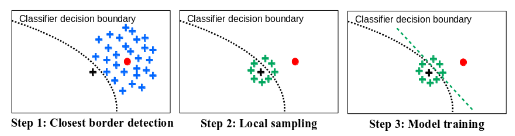
\includegraphics[width=\linewidth]{figure/laugel_method}
		\scriptsize{\textbf{Example:} $\xv$ (red point), closest point from other class (black cross)}
	    %{Local surrogate (LS) method by \citebutton{Laugel et al. 2018}{https://arxiv.org/pdf/1806.07498.pdf}}
		\end{center}
		%Sample new instances $\zv$ around the decision boundary closest from point $\xv$ for higher local accuracy
		% \pause
		% \item Red dot (right figure): Closest point from other class

		% \item Red line: Local surrogate (LS) method \citebutton{Laugel et al. 2018}{https://arxiv.org/pdf/1806.07498.pdf}\\
		% $\leadsto$ better approximates the local direction of the decision boundary 
    \item LIME: What does the model do around this point?
    \item LS: How does the model change when crossing the boundary near this point?
	\end{itemize}

% 	\begin{center}
% 		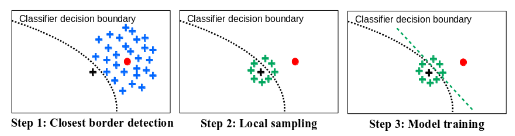
\includegraphics[width=1\textwidth]{figure/laugel_method}
% 	    {Local surrogate (LS) method by \citebutton{Laugel et al. 2018}{https://arxiv.org/pdf/1806.07498.pdf}}
% 		\vspace{-0.3cm}
% 		\end{center}
% \end{column}
% \begin{column}{0.39\textwidth}
% %\vspace{0.3cm}

% 	\begin{center}
% 	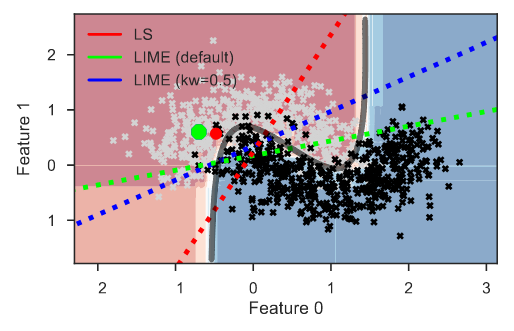
\includegraphics[width=1\textwidth]{figure/lime-globallocal2}
	
% 	{Half-moons dataset}
	
% \end{center}

% 	\end{column}

% \end{columns}
%\footnote[frame]{Laugel et al. (2018). Defining Locality for Surrogates in Post-hoc Interpretability. \url{https://arxiv.org/pdf/1806.07498.pdf}.}
\end{frame}

\begin{frame}{Pitfall: Local vs. Global Features -- Example}
\begin{itemize}
		\item Random forest (RF) classification on half-moons dataset
		    \item \textbf{Background color:} Classification of RF (prediction surface)
		    \item \textbf{Black/grey crosses:} training data
            \item \textbf{Green dot:} Obs. to be explained; \textbf{Red dot:} nearest point from opposite class
		    \item \textbf{Grey curve:} RF's decision boundary; \textbf{Dotted lines:} LIME decision boundaries
             \item \textbf{Red line:} Local surrogate (LS) method \citebutton{Laugel et al. 2018}{https://arxiv.org/pdf/1806.07498.pdf}
	\end{itemize}

    
\begin{columns}[T, totalwidth=\textwidth]
  \begin{column}{0.63\textwidth}
	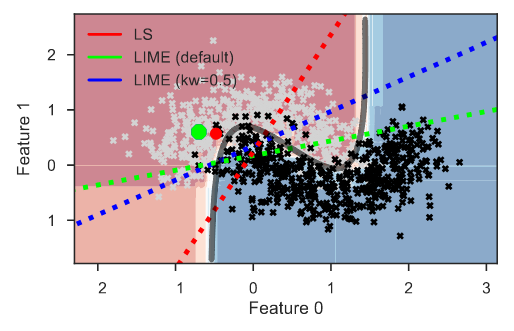
\includegraphics[width=\textwidth, trim = 5px 5px 0px 10px, clip]{figure/lime-globallocal2}
  \end{column}
  \pause
  \begin{column}{0.37\textwidth}
  %\begin{itemize}
  %\item
  \textbf{Feature 0} is global;
  class always flips when moving left (red) to right (blue)
  %\item 
  \medskip
  
  \textbf{Feature 1} is local;
  class flips only near boundary when moving up/down
  %\item Image Source: \citebutton{Laugel et al. 2018}{https://arxiv.org/pdf/1806.07498.pdf}
  %\item 
\medskip

\textbf{Observation:} LIME decision boundaries (blue/green) fail to match the steep local boundary captured by LS (red)
%\end{itemize}

    % \begin{itemize}
    %   \item \textbf{Feature 0} is global; class flips from left (red) to right (blue)
    %   \item \textbf{Feature 1} is local; class flips only in a narrow band around boundary when moving up or down
    % \end{itemize}
  \end{column}
\end{columns}
        
% \begin{center}
%LIME decision boundaries with different kernels (blue and green lines) do not match the direction of the local decision boundary (which appears steeper)
%\footnote[frame]{Laugel et al. (2018). Defining Locality for Surrogates in Post-hoc Interpretability. \url{https://arxiv.org/pdf/1806.07498.pdf}.}
\end{frame}



\begin{frame}{Pitfall: Faithfulness}
\begin{itemize}
%\itemsep1em
	\item \textbf{Problem}: Trade-off between local fidelity vs. sparsity
	\item \textbf{Observation}:
    \begin{itemize}
        \item Too simple model $\leadsto$ low fidelity $\leadsto$ unreliable explanations
        \item Complex model $\leadsto$ high fidelity $\leadsto$ difficult to interpret surrogate %surrogate model cannot easily be interpreted
    \end{itemize}
	\pause
	\item \textbf{Example: Credit data} 
	\begin{itemize}
	\itemsep0em
	    \item Random forest prediction for $\xv$: 
	    $\fh(\xv) = \hat{\P}(y = \text{bad} ~|~ \xv) = 0.143$
	    \item %Regularized linear model with only three selected features (\code{sex}, \code{checking.account}, \code{duration}) $g_{lm}(\xv) = 0.283$
	    Sparse LM with 3 features (\code{age}, \code{checking.account}, \code{duration}):
	    $$\gh_{lm}(\xv) = \thetah_0 + \thetah_1 x_{age} + \thetah_2 x_{checking.account} + \thetah_3 x_{duration} = 0.283$$
	    \item Generalized additive model (with all 9 features) is more complex:
    $$%\begin{equation*} 
    %\begin{split}
    \gh_{gam}(\xv) = \thetah_0 + f_{1}(x_{age}) + f_{2}(x_{checking.account}) + f_{3}(x_{duration}) +  \dots %& = \thetah_0 + s_{age}(x_{age}) +s_{credit.amount}(x_{credit.amount}) s_{duration}(x_{duration}) + \thetah_{sex = male} \ind_{sex = male}   \\
    %& + \thetah_{job}(x_{job}) + \thetah_{housing = own} \ind_{housing = own} +   \thetah_{housing = rent} \ind_{housing = rent} \\
    %& + \thetah_{saving.accounts = moderate} \ind_{saving.accounts = moderate} + \thetah_{saving.accounts = rich} \ind_{saving.accounts = rich} \\
    %& + ... + \thetah_{purpose = radio/TV} \ind_{purpose = radio/TV}  
    = 0.148$$
    %\end{split}
    %\end{equation*}
	\end{itemize}
\end{itemize}

\end{frame}

\begin{frame}{Pitfall: Hiding biases \citebutton{Slack et al. 2020}{https://arxiv.org/abs/1911.02508}}

\begin{itemize}
	% \item \textbf{Problem}: Developer could manipulate their model to hide biases 
	% \item \textbf{Observation}: LIME can sample out-of-distribution points (extrapolation)
      \item \textbf{Problem:} LIME samples out-of-distribution (OOD) points, making it exploitable
  \item \textbf{Risk:} Developers can adversarially hide bias in the original model
	\pause
	\item \textbf{Attack} with adversarial model:
	    \begin{enumerate}
	    \item Train a detector to distinguish in-distribution vs. OOD points
        %classifier to discriminate between in-distribution and out-of-distribution data points
	    %\item for in-distribution points, use the original (biased) model
        \item Use \textbf{biased model} for in-distribution inputs (i.e., true predictions)
	    %\item for out-of-distribution points produced for local explanation, use an unbiased model
        \item Use \textbf{unbiased model} for OOD samples to produce LIME explanations
        \item[$\leadsto$] LIME explanations rely on unbiased model $\Rightarrow$ hides bias in original model 
	    % \item[$\leadsto$] LIME samples out-of-distribution points and uses the unbiased model for local explanation\\
	    % \item[$\leadsto$] this hides the bias of the true model
	    \end{enumerate}
\end{itemize}
%	\begin{columns}[T, totalwidth=\textwidth]
%		\begin{column}{0.5\textwidth}
	    \centering
	    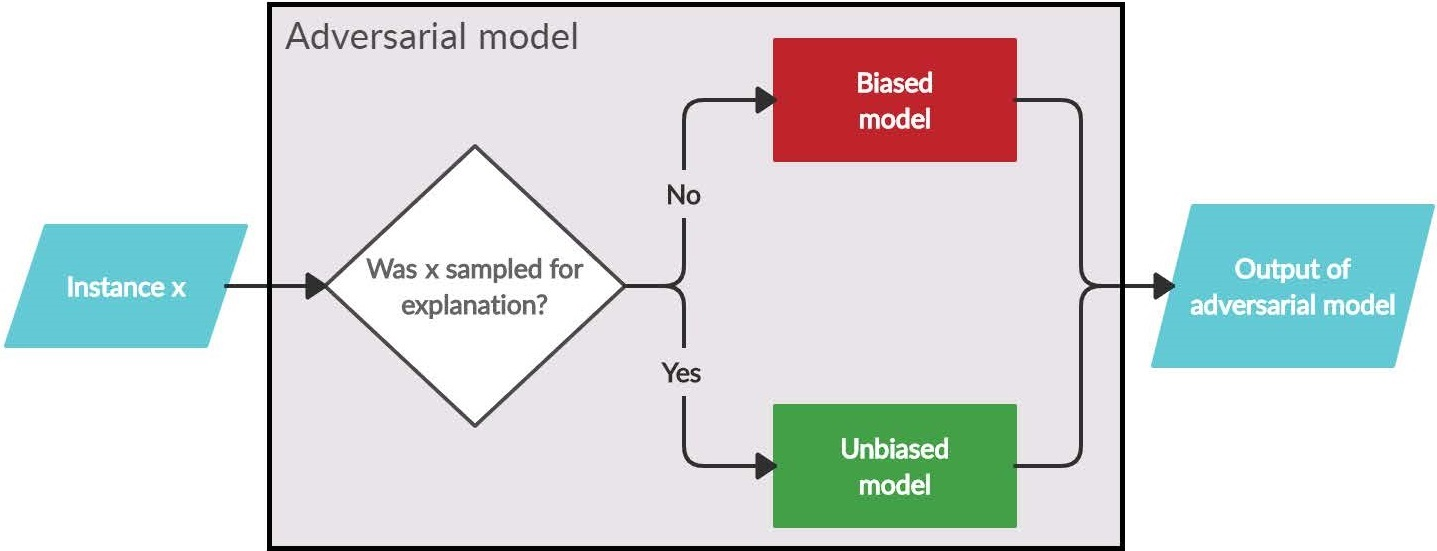
\includegraphics[width=0.85\textwidth]{figure/attack_biased_unbiased.jpg}\\
	    Image Source: \citebutton{Vres, Sikonja (2021)}{https://arxiv.org/abs/2101.11702}
%	    \end{column}
%\pause
	%     \begin{column}{0.5\textwidth}
	%     \textbf{Example}: Not using `gender` to approve a loan % Credit dataset %
	%     \begin{itemize}
	%         \item biased model trained on features correlated with `gender` (e.g. duration of parental leave)\\
	%         $\leadsto$ used 
	%         %for in-distribution points (realistic values) 
	%         to make biased / unfair predictions
	%         \item unbiased model trained on features uncorrelated with `gender`\\
	%         $\leadsto$ used to produce explanations based on unbiased predictions to hide bias
	%         %$\leadsto$ used for (extrapolated) LIME samples\\
	%         %$\Rightarrow$ produced local explanations seem fair as they are based on unbiased model
	%         %could be trained on features uncorrelated with `gender`
	%     \end{itemize}
	%     \end{column}
	% \end{columns}
\end{frame}



\begin{frame}{Pitfall: Hiding biases \citebutton{Slack et al. 2020}{https://arxiv.org/abs/1911.02508}}

\textbf{Key insight:} LIME can be fooled if explanations rely on model behavior outside the true data manifold.

\lz
   
\textbf{Example:} Credit approval
  \begin{itemize}
    \item Biased model uses features correlated with gender (parental leave duration)\\
    $\leadsto$ used to make biased/unfair predictions
    \item Unbiased model uses only features unrelated to gender for fairness\\%omits these correlations
    $\leadsto$ used to produce explanations based on unbiased predictions to hide bias
    \item LIME’s extrapolated samples trigger the unbiased model\\
    $\Rightarrow$ explanation appears fair, but original predictions are biased
  \end{itemize}

\end{frame}











\begin{frame}{Pitfall: Robustness \citebutton{Alvarez-Melis, D., \& Jaakkola, T. 2018}{https://arxiv.org/abs/1806.08049}}
\begin{itemize}
	\item \textbf{Problem}: Instability of LIME explanations 
	\item \textbf{Observation}: Explanations of two very close points could vary greatly 
	\begin{itemize}
	    \item[$\leadsto$] Variability driven by the stochastic sampling of $\zv$ for each explanation
        %can happen because of other sampled data points $\zv$
	\end{itemize}
    \item \textbf{Example:}
\end{itemize}
\vspace{-0.7cm}
\begin{columns}[totalwidth=\textwidth]
	\begin{column}{0.5\textwidth}
		\begin{center}
		
		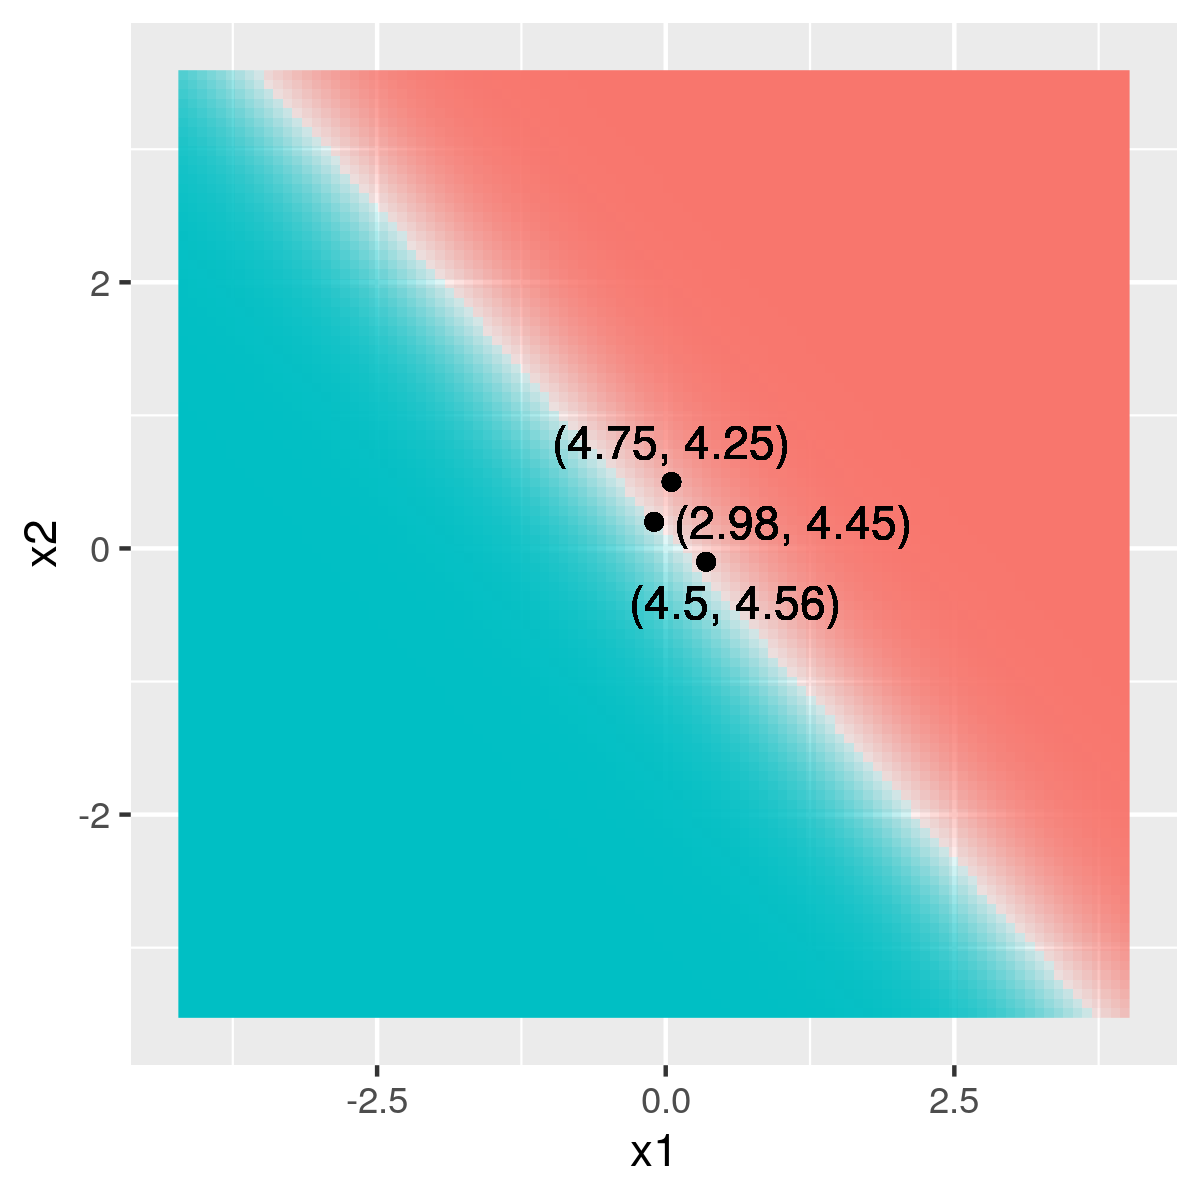
\includegraphics[width=0.8\textwidth]{figure/lime_robustness_1.png}
		
		{Linear task (logistic regression). \\
        LIME returns similar coefficients for similar points.}
		
		\end{center}
	\end{column}
	\begin{column}{0.5\textwidth}
		\begin{center}
	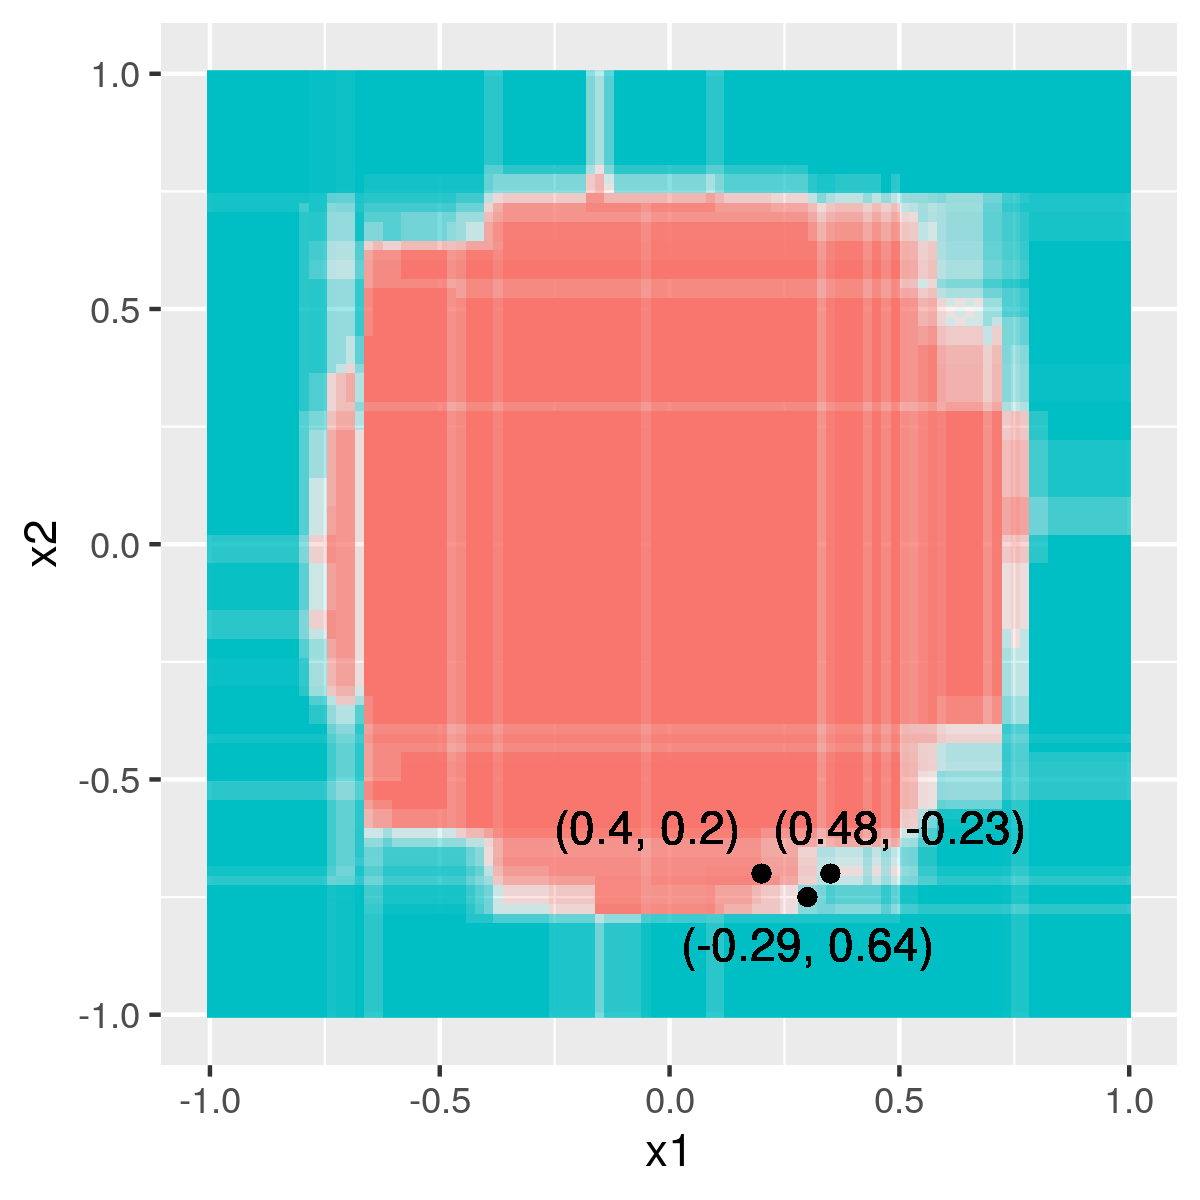
\includegraphics[width=0.8\textwidth]{figure/lime_robustness_2.png}
	
	{Nonlinear task (random forest). 
    \\LIME returns different coefficients for similar points.}
	
	\end{center}
\end{column}
\end{columns}
\end{frame}

\begin{frame}{Pitfall: Definition of Superpixels \citebutton{Achanta et al. 2012}{https://ieeexplore.ieee.org/document/6205760}}

\begin{columns}[totalwidth=\textwidth]
    
    \begin{column}{0.6\textwidth}
        
        \begin{itemize}
        	\item \textbf{Problem}: LIME relies on superpixels (but their definition differ) for image data
            %Instability because of specification of superpixels for image data 
        	\item \textbf{Observation}: Definition of superpixel differ, influencing their size, shape, and alignment 
        	\pause
        	\item \textbf{Implication}: Specification of superpixel has a large influence on LIME explanations 
        	\item \textbf{Attack}: Change superpixels as part of an adversarial attack $\leadsto$ changed explanation
        \end{itemize}
        
    \end{column}
    
    \begin{column}{0.4\textwidth}
    
        \centering
        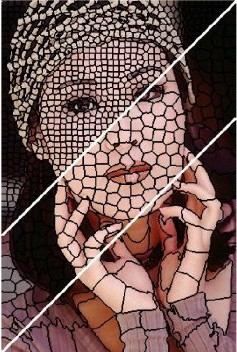
\includegraphics[width=0.7\textwidth]{figure/superpixel_woman}
        
    \end{column}
    
\end{columns}

\end{frame}


\endlecture
\end{document}
